\documentclass[10pt,twocolumn]{article}
\usepackage[letterpaper,margin=0.75in]{geometry}
\usepackage{times}
\usepackage{graphicx}
\usepackage{booktabs}
\usepackage{amsmath,amssymb}
\usepackage{caption}
\usepackage{microtype}
\usepackage[hidelinks]{hyperref}
\captionsetup{font=small,labelfont=bf}
\setlength{\parskip}{2pt}
\newcommand{\pp}{\,pp}

\title{\textbf{Learned Motion Planners Over-Report Success:\\
A Continuous-Feasibility Audit}}
\author{Anonymous\\ \small Workshop submission}
\date{}

\begin{document}
\twocolumn[
\begin{@twocolumnfalse}
\maketitle
\begin{abstract}
Learned and diffusion-based motion planners report success by checking collisions at
the trajectory's \emph{waypoints}. Classical planning has long known this is unsafe --
OMPL recommends continuous (edge) collision checking and cuRobo enforces swept
feasibility by default -- yet learned planners rarely expose the collision-check
resolution behind their headline numbers. We introduce a simple
\emph{resolution-parametrized continuous-feasibility audit}: measure success rate as a
function of the number of collision samples per trajectory edge, $R$. Auditing two
guided-diffusion planners (GPD, EDMP) on the MPiNets Franka benchmark across three
solvability splits (mean$\pm$std over seeds), we find the reported (waypoint) success
rate \textbf{over-states continuous feasibility by $17$--$25\pp$} for the
compact-Bernstein planner (GPD) across all three datasets -- a large fraction of
``collision-free'' plans in fact sweep through obstacles between waypoints. The effect
is \emph{representation-dependent}: for EDMP, whose longer diffusion chain acts on full
50-waypoint trajectories, the gap is small and not significant ($4.2\pm5.2\pp$).
Throughout, \emph{dynamic execution in a physics simulator tracks the dense
static check}, confirming the audit measures a real execution risk. A retraining-free
trajectory-optimization repair makes success nearly \emph{resolution-flat}, closing the
gap. We recommend that learned-planner evaluations report success at a stated,
sufficiently high continuous-check resolution, and release an open audit harness.
\end{abstract}
\vspace{1.0em}
\end{@twocolumnfalse}
]

\section{Introduction}
A motion planner's ``success rate'' (SR) is only as trustworthy as the collision check
behind it. A trajectory that is collision-free at 50 sampled waypoints can still sweep a
7-DoF arm through an obstacle \emph{between} those waypoints -- the classic ``tunnel''
effect. Classical planning treats this as a first-order concern: OMPL's default
\texttt{DiscreteMotionValidator} discretizes each edge at a chosen resolution and its
documentation explicitly recommends a continuous \texttt{MotionValidator} when available
\cite{rrtconnect2000}, and GPU planners such as cuRobo \cite{curobo2023} enforce swept
collision via signed-distance fields by default.

Learned and diffusion-based planners \cite{diffuser2022,mpd2023,edmp2024,gpd2025},
however, typically report SR from a waypoint or coarse execution check and do not expose
the underlying collision-check resolution -- so it is unclear how much of their reported
success survives a continuous check. Differentiable swept-volume models exist
\cite{svsdf2024,neuralsvcd2025} and safe-diffusion methods \cite{safediffuser2025} enforce
constraints at sampled points, but no prior work \emph{measures} how learned-planner SR
depends on collision-check resolution.

We fill this gap with a resolution-parametrized audit and report three findings:
(1) the waypoint$\to$dense SR gap is \textbf{$17$--$25\pp$} for GPD across three
datasets, and is representation-dependent (small/insignificant for EDMP); (2)
\emph{dynamic execution} in PyBullet $\approx$ the dense static check, so the gap is a
genuine execution risk, not a checker artifact; (3) a retraining-free
trajectory-optimization repair makes SR nearly resolution-independent. We recommend reporting SR at a stated continuous-check
resolution and release the harness.

\section{Related Work}
\textbf{Collision checking.} OMPL separates state validity from \emph{motion} validity;
the discrete motion validator samples each edge at \texttt{longest\_valid\_segment}
resolution, a known accuracy/cost trade-off, while continuous checkers avoid it
\cite{rrtconnect2000}. cuRobo \cite{curobo2023} optimizes a continuous swept-volume SDF.
\textbf{Swept-volume models.} Neural/implicit swept-volume representations
\cite{svsdf2024,neuralsvcd2025} provide differentiable continuous collision signals but
are used inside optimization, not to \emph{audit} learned planners.
\textbf{Diffusion planners.} Diffuser \cite{diffuser2022}, MPD \cite{mpd2023}, EDMP
\cite{edmp2024}, and GPD \cite{gpd2025} guide sampling by collision cost and report SR by
executing/checking discretized trajectories; none reports a resolution sweep.
\textbf{Safe diffusion.} SafeDiffuser \cite{safediffuser2025} enforces control-barrier
constraints at sampled points during denoising. Our contribution is orthogonal: an
\emph{evaluation} protocol that quantifies the discrete-check over-reporting these
methods are all exposed to.

\section{The Audit}
Let a planner output a waypoint trajectory $\tau=(q_0,\dots,q_{N})$. For a resolution
$R$ (samples per edge) we linearly densify each edge into $R$ sub-configurations and
declare $\tau$ \emph{$R$-feasible} iff \emph{every} sampled configuration is collision-free
under a faithful checker (PyBullet \texttt{getContactPoints} against the scene). $R{=}1$
recovers the waypoint check; large $R$ approaches true continuous feasibility.
\textbf{Continuous SR@$R$} is the fraction of $R$-feasible plans over a scene set.
We sweep $R\in\{1,2,4,8,16,32\}$ and, as a reference, also report \emph{dynamic}
success: executing $\tau$ under position control and checking contact at every physics
step. We audit each planner's \emph{base} pipeline and its output after a
retraining-free trajectory-optimization \emph{repair} (Adam on interior waypoints
minimizing a differentiable collision cost at waypoints and edge-midpoints, early-stopped
on a densified faithful check \cite{presto2025}).

\noindent\textbf{Setup.} Guided Polynomial Diffusion (GPD, \cite{gpd2025}) and EDMP
\cite{edmp2024} on the MPiNets \cite{mpinets2022} Franka Panda benchmark
(tabletop/cubby/merged-cubby/dresser), on the global/hybrid/both-solvable splits,
balanced per type. SR@$R$ curves are averaged over 5 sampling seeds (GPD hybrid) / 3
seeds (other splits, EDMP); we report mean$\pm$std.

\begin{figure*}[t]
\centering
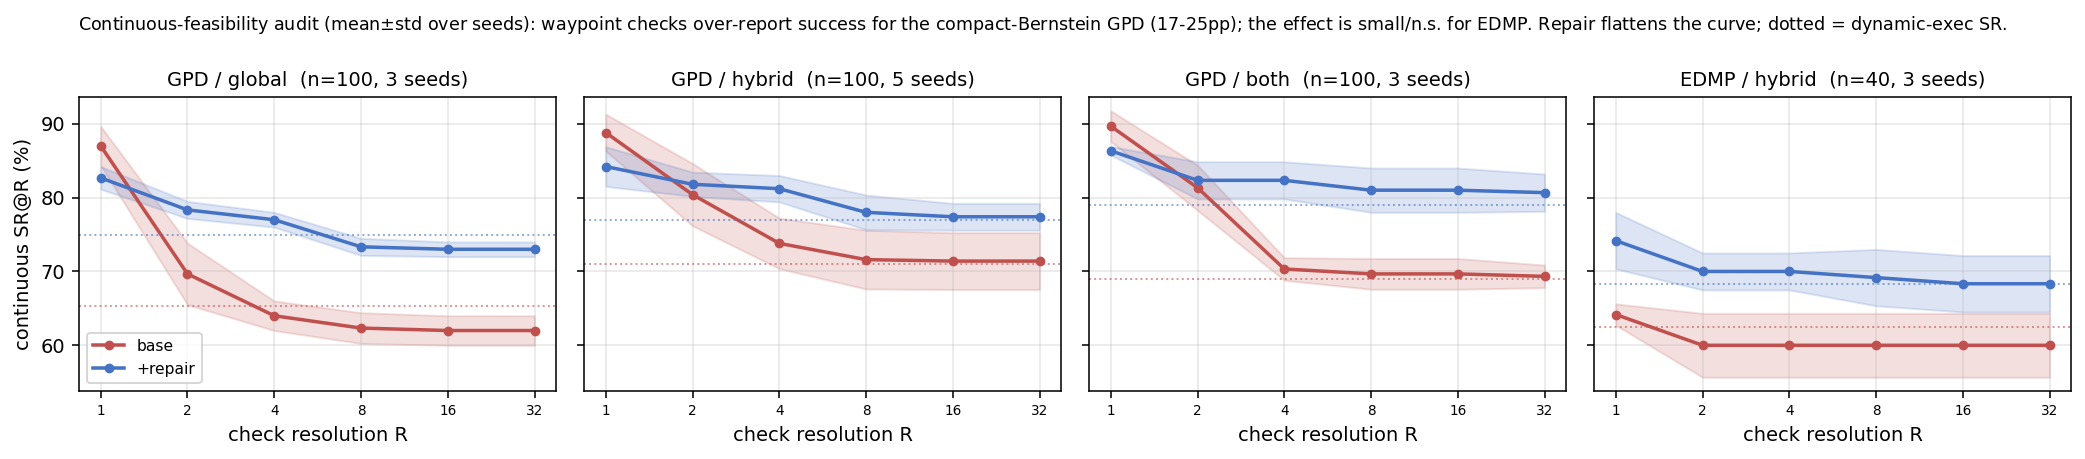
\includegraphics[width=0.98\textwidth]{figs/continuous_audit_cross.png}
\caption{Continuous-feasibility audit across datasets (GPD: global/hybrid/both) and a
second planner (EDMP). \emph{Base} (red) success collapses as the check densifies;
\emph{repair} (blue) is nearly resolution-flat; dotted lines are dynamic-execution SR
($\approx$ the dense static check). The waypoint$\to$dense over-reporting is
$10$--$27\pp$.}
\label{fig:audit}
\end{figure*}

\section{Results}
\textbf{Waypoint checks over-report by $17$--$25\pp$ for GPD (Fig.~\ref{fig:audit}).}
Base continuous SR@$R$ drops sharply from $R{=}1$ (waypoints) to $R{=}32$
(mean$\pm$std over seeds):

\begin{center}\small
\begin{tabular}{lccc}
\toprule
planner / split & SR@1 & SR@32 & over-report \\
\midrule
GPD / global & $87.0{\pm}2.6$ & $62.0{\pm}2.0$ & $\mathbf{-25.0{\pm}1.7}$ \\
GPD / hybrid & $88.8{\pm}2.5$ & $71.4{\pm}3.8$ & $\mathbf{-17.4{\pm}2.6}$ \\
GPD / both   & $89.7{\pm}2.1$ & $69.3{\pm}1.5$ & $\mathbf{-20.3{\pm}1.2}$ \\
EDMP / hybrid & $64.2{\pm}1.4$ & $60.0{\pm}4.3$ & $-4.2{\pm}5.2$ (n.s.) \\
\bottomrule
\end{tabular}
\end{center}

\noindent For GPD, a fifth to a quarter of nominally-``collision-free'' plans sweep
through obstacles between waypoints, and the gap is tight and significant across all
three datasets. The effect is \emph{representation-dependent}: EDMP's longer diffusion
chain over full 50-waypoint trajectories yields denser, smoother inter-waypoint motion,
so its (already lower) success rate barely changes with $R$ ($-4.2{\pm}5.2\pp$, not
significant). The over-reporting is thus a property of the \emph{trajectory
representation and check resolution}, most acute for compact bases like GPD's degree-7
B\'ezier -- exactly the parameterizations favored for speed.

\noindent\textbf{Dynamic execution $\approx$ the dense static check.} In every cell the
dynamic-execution SR lands at the high-$R$ plateau (e.g.\ GPD/both $71\%$ dynamic vs
$71\%$ at $R{=}32$; GPD/hybrid $71$ vs $73$), so SR@high-$R$ is not a pessimistic
artifact -- it predicts what happens when the trajectory is actually run.

\noindent\textbf{Repair closes the gap.} Post-hoc trajectory-optimization makes SR nearly
resolution-flat (e.g.\ GPD/hybrid $84\!\to\!82\%$ from $R{=}1$ to $32$), producing plans
that are \emph{genuinely} continuous-feasible rather than merely waypoint-free. Repair is
retraining-free and planner-agnostic (it also lifts EDMP).

\section{Discussion}
The audit is a cheap, general prescription: \emph{report learned-planner success at a
stated continuous-check resolution} (or under dynamic execution), not at the waypoints
alone -- matching decades-old classical-planning practice. Two practical notes. First,
the fix need not be a heavier objective: in companion experiments a dense
multi-sample-per-edge repair objective did not beat the single-midpoint one, because the
repair early-stops on a densified \emph{faithful} oracle -- the check resolution, not the
differentiable objective, is what matters. Second, the audit is a measurement tool, not a
planner; combined with repair it yields both an honest number and a way to reach it.
\textbf{Limitations.} One robot and one benchmark family; the faithful checker is
PyBullet contact (mesh-level but simulator-specific); $R$ up to 32 approximates but does
not certify continuous feasibility.

\section{Conclusion}
Learned motion-planning success rates depend on an unreported collision-check resolution
and over-state continuous feasibility by $17$--$25\pp$ for a compact-Bernstein planner
across three datasets (representation-dependent; small for EDMP);
dynamic execution confirms the gap; retraining-free repair closes it. We recommend
resolution-parametrized reporting and release an open audit harness.

\small
\bibliographystyle{plain}
\bibliography{refs}
\end{document}
